\documentclass{llncs}

\usepackage{amsmath} % for equation*
\usepackage{color}
\usepackage{hyperref}
\usepackage{graphicx}
\usepackage{stmaryrd}
\definecolor{darkgreen}{rgb}{0,0.7,0}

% Fix link colors
\hypersetup{
    colorlinks = true,
    linkcolor=red,
    citecolor=red,
    urlcolor=blue,
    linktocpage % so that page numbers are clickable in toc
}

\pagestyle{plain}

\newcounter{ques}
\setcounter{ques}{1}

\newcommand{\todo}[1]{\color{blue}\textbf{TODO:} #1\color{black}}
\newcommand{\myspace}[0]{\vspace*{0.25cm}}

\renewcommand{\question}[1]{\paragraph{}\textbf{Q\theques} - #1\stepcounter{ques} }

\newcommand{\answer}[1]{}%\color{red}\textit{#1}\color{black}}
\title{COMP 445 -- Final exam \\ Winter 2017 \\ Friday, April 28, 2017 \\ Duration: 180 minutes}

\author{Tristan Glatard\\
  \href{mailto:tristan.glatard@concordia.ca}{tristan.glatard@concordia.ca}\\
  \vspace*{0.3cm}
  }

\institute{Concordia University\\
  Department of Computer Science and Software Engineering}

\begin{document}

\maketitle

\section*{Instructions}
\begin{itemize}
\item All questions will receive equal points.
\item Answer all questions on these sheets in the space provided.
\item No books, notes or extra paper.
\item No cell phones, laptops or any electronic devices except ENCS calculators.
\item This exam is 21 pages long, including the cover page. It has 20 questions labeled from \textbf{Q1} to \textbf{Q20} (one question per page except on this cover page). Check that your copy is complete.
\item This exam counts for 50\% of your final grade.
\end{itemize}

\myspace

\myspace

\hrulefill\\

\myspace

Consistent with the university regulations concerning cheating and plagiarism I will not cheat during this examination:

\myspace

\myspace

Student ID: \dotfill

\myspace

\myspace

First Name / Last Name: \dotfill

\myspace

\myspace

Signature: \dotfill

\myspace

\myspace

\hrulefill

\newpage

\section{Introduction}

% 2 questions

\question{List the layer(s) of the internet protocol stack that are implemented
  at the network edges, i.e., not at the core. For each layer, list
  two protocols.}

\answer{
\begin{itemize}
\item Application: HTTP, SMTP.
\item Transport: TCP, UDP. 
\end{itemize}
}

\newpage

\question{Explain the principle of packet encapsulation. Give an
  example using protocols of the internet protocol stack. }

\answer{ Packet encapsulation is the process according to which the
  packet produced by layer $n-1$ is formed by appending a header and
  possibly a trailer to the packet produced at layer $n$.  For
  instance, the IP header is appended to a TCP segment to form an IP
  datagram.}

\newpage

\section{Application Layer}

% 2 questions

\question{List two HTTP method types and explain their behavior.}

\answer{
  \begin{itemize}
  \item GET: get the content at a URL.
  \item POST: send data to a URL.
  \item HEAD: get the header lines only, not the requested object.
  \end{itemize}
}

\newpage

\question{The content below was captured using
  Wireshark:\\
  
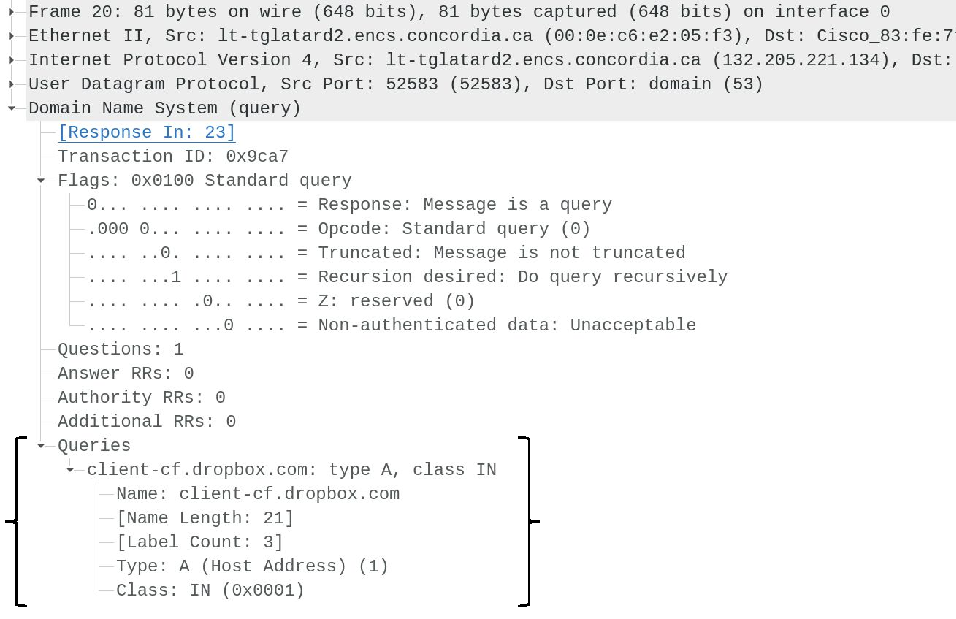
\includegraphics[width=\textwidth]{dns.png}

\begin{enumerate}
\item What is the application-level protocol in this content?
\item What is the transport-level protocol in this content?
\item What is the meaning of the ``Queries'' section in the last 7 lines? 
\item Is this content coming from a client or from a server?
\item Describe a possible follow-up message for this content, i.e.,
  how the client or server may respond to this message. Only a
  high-level description of the message is expected, i.e., you don't
  have to write the complete message explicitly.
\end{enumerate}
}

\answer{
  \begin{itemize}
  \item DNS
  \item UDP
  \item It is a DNS query, asking for the IP of host with name ``client-cf.dropbox.com''.
  \item From a client as it has no answers.
  \item A DNS response might be sent to the client, containing the requested IP. 
  \end{itemize}
}

\newpage

\section{Transport Layer}

% 2 questions

\question{Explain the main differences between UDP and TCP (at least
  two differences are required). Explain why an application may choose
  UDP over TCP (only 1 reason is required).}

\answer{ TCP provides reliable data transfer, connections, flow control and
  congestion control while UDP does not provide any of them. An
  application may choose UDP to avoid overheads related to reliable
  data transfers and to avoid throttling due to congestion control.}

\newpage

\question{Explain the meaning, setting and use of the TCP timeout, more precisely:
  \begin{itemize}
  \item when do timeout events occur? 
  \item how is the timeout value set? (a formula is expected)
  \item what happens when a timeout occurs?
  \end{itemize}
}

\answer{
  \begin{itemize}
  \item See slide 54. Timeout events occur when acknowledgements are not received in time.
  \item See slides 62 and 63. Timeout = EstimatedRTT + 4*DevRTT and EstimatedRTT=(1-$\alpha$)*EstimatedRTT+$\alpha$*SampleRTT.
  \item See slide 104. The slow start threshold is divided by 2, the congestion window is set to 1 MSS, the duplicate ACK count is set to 0, the missing segment is retransmitted.     
  \end{itemize}
}

\newpage

\section{Network Layer}

% 5 questions

\question{Explain the primary goal of the Time To Live (TTL) field in
  the IPv4 datagram header. Explain how this field is also
  used to trace network routes on the internet (tracing routes is not
  the primary goal of the TTL).}

\answer{The primary goal of TTL is to prevent datagrams from
  circulating forever in the network, for instance in case of routing
  loops among routers. The TTL is decremented by each router. When it
  reaches 0, the router destroys the datagram and sends an ICMP
  message to the source. To trace the route between a source and a
  destination, the traceroute program sends datagrams with increasing
  TTLs (starting at 1) so that it receives ICMP messages from all the
  routers on the path to the destination and can thus retrieve their
  IP addressesx. }

\newpage

\question{What is the subnet address associated with IP address
  172.30.123.47/24?}

\answer{The \texttt{/24} suffix indicates that the first 24 bits,
  i.e. 3 bytes, are allocated to the subnet. Therefore the subnet
  address is 172.30.123.0.}

\newpage
  \setlength{\tabcolsep}{12pt}
\question{\underline{Using the Dijkstra algorithm}, compute the least-cost
  paths from A to all the other nodes in the graph below. Your answer
  will have to detail the successive iterations of the algorithm.}

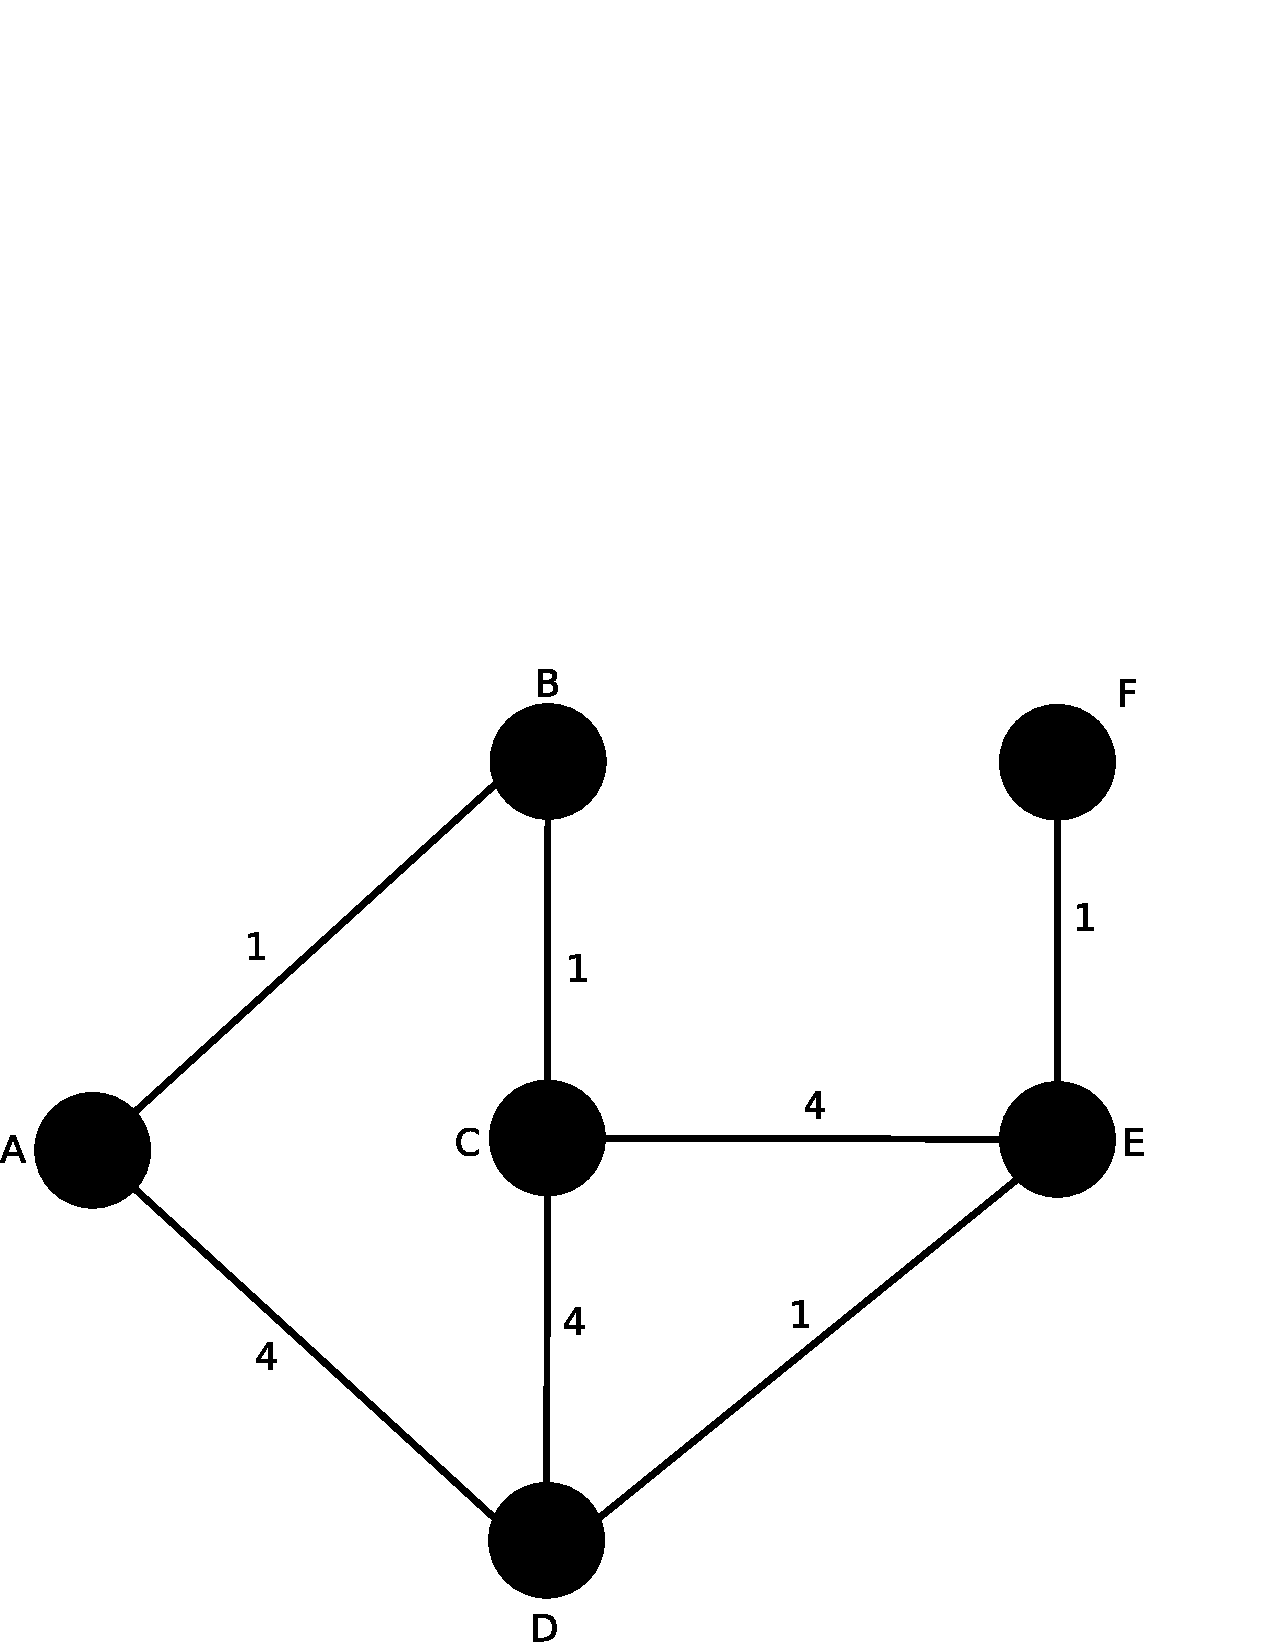
\includegraphics[width=0.5\textwidth]{graph.pdf}

\answer{
  The following table uses the notations on slides 79-80 of the lecture on the Network Layer.\\
  \begin{tabular}{lccccc}
    N'     & B   & C        & D   & E        & F        \\
    A      & \underline{1,A} & $\infty$ & 4,A & $\infty$ & $\infty$\\
    AB     &     & \underline{2,B}      & 4,A & $\infty$      & $\infty$     \\
    ABC    &     &          & \underline{4,A} & 6,C      & $\infty$    \\
    ABCD   &     &          &     & \underline{5,D}      & $\infty$     \\
    ABCDE  &     &          &     &          & \underline{6,E}     \\
    ABCDEF &     &          &     &          &                     \\
     \end{tabular}
}


\newpage

\question{Routing Information Protocol (RIP). Starting from the initial
  RIP table in C shown below, suppose that C receives from A the following
  advertisement. Will the table in C change? If so how?
  \begin{itemize}
\item  Original RIP table in C:\\
\begin{tabular}{ccc}
  Destination subnet & Next router & Hops to destination \\
  \hline
  u & - & 1\\
  v & D & 2\\
  w & - & 1 \\
  x & F & 4\\
\end{tabular}
\item \vspace*{1cm}Advertisement received by C from A:\\
\begin{tabular}{ccc}
  Destination subnet & Next router  & Hops to destination\\
  \hline
  u & C & 2\\
  v & B & 3\\
  w & - & 1 \\
  x & B & 2\\
\end{tabular}
\end{itemize}
}

\answer{New table in C:\\
  \begin{tabular}{ccc}
    Destination subnet & Next router & Hops to destination \\
    \hline
    u & - & 1\\
    v & D & 2\\
    w & - & 1\\
    x & \textbf{A} & \textbf{3}\\
  \end{tabular}
}


\newpage

\section{Link Layer}

% 4 questions

\question{Carrier-Sense Multiple Access (CSMA) is a multiple-access
  protocol where hosts listen to the channel before transmitting and
  do not transmit if the channel is sensed busy. Explain why
  collisions may still occur on a shared channel that uses this
  protocol.}

\answer{Collisions may still occur with CSMA because of propagation
  time on the shared channel. When a host A senses the channel,
  another host B may have been transmitting for a duration shorter
  than the propagation time between A and B. Therefore, A is not able
  to detect B's transmission and will therefore transmit its own data,
  leading to a collision. See slide 30. }

\newpage

%\question{Give an example of a MAC address. What is the protocol used
%  to determine the MAC address of a host from its IP address?}

\question{What is the exponential backoff in Ethernet's CSMA/CD
  algorithm? Explain why it involves pseudo-random numbers (what would
  happen if no randomness was involved).}

\answer{See slide 33. CSMA/CD's exponential backoff determines the duration a host
  has to wait after a collision was detected. After m collisions, a
  random number K is chosen in $\llbracket 0,2^m-1 \rrbracket$ and the
  host waits for K.512 bit times, where a bit time is the time to
  transmit a bit on the channel. If no randomness was involved, hosts
  would retransmit at similar times after a collision, which would
  lead to another collision with high probability.}


\newpage

\question{A switch is a self-learning device, i.e., it discovers the
  MAC addresses that can be reached from its interfaces. Using
  a simple example, explain how such a self-learning process works.}

\answer{A switch maintains a table that matches MAC addresses to
  interfaces. When it receives a frame, it adds the source MAC address
  of this frame to the table with the interface on which the frame was
  received. A TTL is also added to remove entries after a certain
  amount of time. In this way, switches learn the interfaces on which
  MAC addresses can be reached as frames are being sent from this MAC addresses.}

\newpage

\question{Synthesis: list three types of host addresses used in the
  internet protocol stack. Explain the rationale for each address
  type, i.e., why it is required or useful in the internet. Show an
  example of each address type. List and briefly describe the
  corresponding address resolution protocols.}

\answer{ DNS names, IP addresses and MAC addresses are three types of
  host addresses used in the internet protocol stack.  The rationale
  for DNS is to provide human-readable names that are easy to
  remember, for instance \texttt{www.concordia.ca}. IP addresses are
  designed to facilitate routing at the global internet scale since
  prefixes identify sub-networks. An example of an IP address is
  \texttt{172.30.102.135}. MAC addresses identify a physical
  device. They are independent from the location of a host while the
  IP address of a host changes when the host changes network. An example of a MAC address is \texttt{f0:d5:bf:50:80:98}. Address resolution protocols are:
  \begin{itemize}
  \item DNS: to map DNS names to IP addresses.
  \item ARP: to map IP addresses to MAC addresses. 
  \end{itemize}
}
% Add IPv6

\newpage

\section{Security}

% 5 questions

\question{Compare symmetric and asymmetric cryptography by listing at least one
  advantage of each method over the other one.}

\answer{Symmetric cryptography is faster than asymmetric
  cryptography. However, symmetric cryptography requires a shared
  secret to be sent over a secure channel while asymmetric
  cryptography does not. }

\newpage

\question{In the RSA algorithm, assume that the public key is (35,5)
  and the private key is (35,29). That is, n=35, e=5 and d=29. Using
  the public key, encrypt the message represented by decimal
  number 17. Then, show how the ciphered message can be decrypted.}

\answer{See slide 23. Encryption: $17^{5}\quad \mathrm{mod}\quad 35 =
  12$. Decryption: $12^{29}\quad \mathrm{mod}\quad 35 = 17$.}

\newpage

\question{What is a cryptographic hash function? Give an example of
  protocol or situation where it is useful (1 example expected).}

\answer{A cryptographic hash function is a many-to-1, one-way function
  that produces a fixed-size digest from a message of arbitrary
  size. Hash functions are used for digital signatures so that only a
  short message digest has to be encrypted with asymmetric
  cryptography.}

\newpage

\question{Explain the principles of digital signature, using an
  example where Alice signs a document and sends it to
  Bob.}

\answer{See slide 50. When Alice wants to sign a document, the
  signature consists of the document digest encrypted with Alice's
  private key. When Bob receives the signed document, he (1) computes
  its digest and (2) decrypts the signature using Alice's public
  key. If the results of (1) and (2) match, the document's signature
  is verified.}

\newpage

%% \question{SSL, IPSec and WPA (802.11i) are three security protocols. List the
%%   layers in the internet protocol stack where each of these protocols
%%   belongs. Explain why there is a need for three different
%%   protocols by describing, for each protocol, a situation where the other
%%   two protocols cannot be used or do not provide the required service.}

\question{What is the purpose of a random nonce? Give an example of a
  protocol that uses nonces and explain where they are used in the
  protocol. }

\answer{A nonce is a number used only once in a lifetime. It is used
  to protect against playback attacks where an attacker replays the
  exact same sequence of events than in a previous communication. SSL
  uses nonces in its handshake, to guarantee that encryption and MAC
  keys will be different for every session.  }


\newpage

\question{Consider an \texttt{echo} server such as the one in the code
  examples of the first lab assignment (LA1). This server listens for
  incoming TCP connections, for instance on port 1234, and sends back
  an identical copy of any content it receives through a given
  connection. \underline{Without modifying the code of this server},
  how would you ensure that only the hosts of a particular sub-net can
  access it?}

\answer{Use a firewall to filter incoming packets from any host except
  the ones on the sub-net.}

\end{document}
